In this section we will introduce our reference implementation (henceforth
sometimes called the \emph{package grabber scenario}), which we have
developed to showcase and test our engine. It will also serve as an
example of using the engine as well as the extensions we have provided.
In section \ref{sec:ImplementationReferenceImplementation}, we will
detail the actual implementation of the scenario in the engine, the
agent programs, as well as the integration of the two. A less complex
example, which describes the simple vacuum world (~\cite{Norvig96},
p.\ 35), can be found in appendix\texttt{\emph{ \ref{chap:VacuumWorldAppendix}}}.

The reference implementation is intended to cover as many of the engine
features and extensions as possible, while not focusing on creating
any particularly revolutionary artificial intelligence. As such, we
have set up a world that is relativively simple with respect to the
action and perception repetoire of the agents, and with an environment
representation limited in complexity. Thus, the interesting part of
the reference implementation is not the scenario itself, but rather
the actual implementation. That being said, the scenario is as follows:

\begin{figure}
\begin{centering}
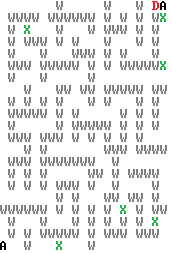
\includegraphics[width=0.4\textwidth]{TileWorldColoredScrot}
\par\end{centering}

\caption{An initial configuration of the package grabber scenario. \texttt{D}
(red) marks the dropzone, \texttt{X}s (green) are packages, \texttt{A}s
(black) are agents and \texttt{W}s (grey) are walls\label{fig:maze-scrot}}
\end{figure}


The agents in the scenario are tasked with exploring a maze in a discrete
two dimensional grid of tiles in order to locate \texttt{package}s
and bring them to a special tile called the \texttt{dropzone} (see
figure \ref{fig:maze-scrot}). A tile in this scenario can contain
several objects, unless they are explicitly forbidden to occupy the
same square. An agent, for example, can not move into a tile that
already contains another agent, but it can move into a square containing
a package or a dropzone. Importantly, a tile containing a \texttt{wall}
cannot contain anything else, thus the tiles between walls constitutes
the navigable pathway of the maze. 


\subsection*{Actions}

The three actions \emph{moving}, \emph{grabbing} and \emph{dropping}
are enough for the agents to fulfill their task, and as such they
describe the complete action specification:
\begin{description}
\item [{\texttt{move(}\texttt{\emph{Direction}}\texttt{)}}] moves the agent
one tile in the specified \texttt{\emph{Direction}}. \texttt{\emph{Direction}}\emph{
}is limited to the four cardinal directions, so an agent can only
move to an immediately adjacent square. Note that every tile not containing
a wall is reachable from every other such tile in the maze when following
this movement rule.
\item [{\texttt{grab}}] removes the package in the same tile as the agent
(if any) from the world, and marks the agent as carrying a package.
\item [{\texttt{drop}}] adds a package to the world in the same tile as
the agent (if it is carrying a package) and marks the agent as not
carrying a package. If a package is dropped at a dropzone, it is removed
from the world.
\end{description}
Note that this action specification does not mention any means of
communicating or otherwise cooperating, which is an otherwise important
feature of any multi-agent system. We have not implemented such functionality
in the XMAS engine, although it would be a high priority task if we
were to develop it further. Normally, GOAL provides built-in communication
devices, which we cannot use in the reference implementation, for
reasons explained in the implementation section. In general, although
several grabber agents can inhabit the scenario, they will not actively
work together or compete, although they will try to accomplish the
same goals.


\subsection*{Percepts}

\begin{figure}
\begin{centering}
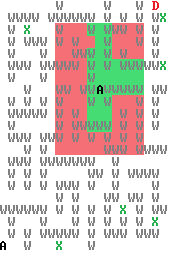
\includegraphics[width=0.4\textwidth]{TileWorldColoredScrotVision}
\par\end{centering}

\caption{Here we see the visible tiles for the agent in the middle of the colored
section. Tiles colored in green are visible to the agent while tiles
in red are are blocked by walls. All other tiles are outside the agents
visibility range, and thus invisible. As can be seen, agents are good
at peeking around corners.\label{fig:maze-scrot-vision}}


\end{figure}


Now that agents can act in the environment, they must also be able
to sense their surroundings in order to make informed choices about
their course of action. For this purpose, the following three percepts
can be obtained from the world:
\begin{description}
\item [{Vision:}] A rather obvious perception device in this scenario is
\emph{vision}, allowing an agent to learn the contents of tiles around
it. Each agent can can see a distance of five tiles in any direction,
assuming there is no walls or other agents blocking its vision. See
fig. \ref{fig:maze-scrot-vision} for an illustration.
\item [{Package~Possession:}] Specifies whether the agent is currently
holding a package. An agent can only hold one package at a time. This
truth value could be mangaged by the agent program, but having it
as a percept is easier on the AP. Additionally, an effect could forcibly
remove a package from an agent, and we would thus need a percept for
that (note that such an effect does not currently exist in the scenario).
With our current approach, we provide a snapshot of the state of the
perceivable world through percepts and let the AP make of it what
it can.
\item [{Position:}] The absolute position of the agent in the grid. In
the agent program, we initially used positions relative to the starting
position of the agent to build a map of maze. However, using this
method we would lose track if the agent was forcibly pushed into another
tile (again, such an effect does not exist in this scenario).
\end{description}
Additionally, agents receive their current movement speed (the time
it takes to move from one tile to an adjacent one) as a percept, although
we do not use it in this scenario.


\subsection*{Agent Program}

We have implemented the agent logic for the grabber agent in the GOAL
agent programming language. The GOAL instance is connected to an EIS
environment, which communicates with the XMAS engine by sending actions
and receiving percepts.

It will try to find all packages in the maze and bring them to the
dropzone. Note that since packages might be hidden in places the agent
has not yet looked, the requirement for scenario completion is not
just that no more packages can be \emph{seen }on the map, but also
that there are no more tiles to explore.

In order to find all the hidden packages, the agent must explore the
maze by moving to tiles it has not stood on before in order to gain
vision of other tiles and pathways. The agent logic itself is pretty
straight forward; it can be summarized as below:

\begin{alltt}
\textit{if} I hold a package 
        \textit{and} know the location of the dropzone
    \textit{then} go to the dropzone and drop it
\textit{if} I have no package 
        \textit{and} know the location of one 
    \textit{then} go grab the package
\textit{otherwise}, 
    explore the maze further
\end{alltt}

In the pseudo code above, decisions such as ``\texttt{explore the
maze further}'' are \emph{goals} the agent sets for itself. When
it needs to get to a specific location, it finds a path to that location
using the \texttt{A{*}} algorithm, and then follows it each turn until
it reaches a goal or finds something better to do.
